%==============================================================================
% Safe but Slow -- IEEE conference paper (IEEEtran, two-column)
%
% Build:  pdflatex main  ->  bibtex main  ->  pdflatex main  ->  pdflatex main
% The class file IEEEtran.cls and the style IEEEtran.bst ship with TeX Live and
% with Overleaf; no other file is needed beyond refs.bib and figs/*.pdf.
%==============================================================================
\documentclass[conference]{IEEEtran}
\IEEEoverridecommandlockouts

\usepackage{cite}
\usepackage{amsmath}
\usepackage{amssymb}
\usepackage{graphicx}
\usepackage{booktabs}
\usepackage{array}
\usepackage{xcolor}
\usepackage{tikz}
\usetikzlibrary{arrows.meta,positioning,calc,fit,backgrounds}
\usepackage[hidelinks]{hyperref}
\usepackage{url}

\graphicspath{{figs/}}

% Marks a result that is planned but not yet measured, so a reader never takes a
% placeholder for a finding.
\newcommand{\wip}{\textsuperscript{\textcolor{orange!80!black}{$\ast$}}}
\newcommand{\wipnote}{\textsuperscript{\textcolor{orange!80!black}{$\ast$}}\,in progress}

% Figure colours, kept in step with figs/make_figures.py.
\definecolor{fblue}{HTML}{2A78D6}
\definecolor{forange}{HTML}{EB6834}
\definecolor{faqua}{HTML}{1BAF7A}
\definecolor{fink}{HTML}{52514E}

\begin{document}

\title{Safe but Slow: Objective Labels for\\Over-Conservative Driving Trajectories}

\author{\IEEEauthorblockN{Yiqi Su}
\IEEEauthorblockA{\textit{Institute of Industrial Science} \\
\textit{The University of Tokyo}\\
Tokyo, Japan \\
su.y@t2.auto}
\and
\IEEEauthorblockN{Kimihiko Nakano}
\IEEEauthorblockA{\textit{Institute of Industrial Science} \\
\textit{The University of Tokyo}\\
Tokyo, Japan}
}

\maketitle

\begin{abstract}
Learned planners are trained to copy a human drive, so a hesitant drive is copied
as faithfully as a decisive one. Work that adds negative examples to imitation
learning has so far used unsafe trajectories, which leaves a second failure mode
unaddressed: waiting when there is nothing to wait for. This paper gives a
computable definition of that failure mode. A trajectory is treated as
over-conservative when it is safe by the usual measures and clearly slower than
the human drive, provided no traffic-engineering reason for the delay can be
found. Two independent tests supply the reason. One asks whether the slower
trajectory turned down a gap that drivers are known to accept, using critical
gap values from the Highway Capacity Manual. The other asks whether a vehicle
hidden behind an obstruction could have reached the conflict point first. On the
NAVSIM navtest split the procedure labels 2{,}783 trajectories across 742
scenes without any human annotation. The occlusion test alone accounts for 207
of the 244 scenes it protects, so it is not redundant with the gap test. A
camera-only Latent TransFuser baseline scores 94.3 on the benchmark metric in
unsignalized crossings, its best stratum, yet accepts only 30\% of the gaps a
human accepted there, which shows the benchmark metric does not see this
failure. Training with the labels is under way.
\end{abstract}

\begin{IEEEkeywords}
autonomous driving, motion planning, imitation learning, gap acceptance, occlusion
\end{IEEEkeywords}

%==============================================================================
\section{Introduction}
%==============================================================================

A planner that never collides is not yet a planner one would want to ride
behind. In merges and unprotected turns the vehicle has to weigh safety against
acting in time, and worst-case reasoning tends to settle that trade-off by
waiting~\cite{trautman2010,schwarting2019}. The cost is real. Hesitation delays
the traffic behind and makes the vehicle's intent hard for other drivers to
read.

Imitation learning inherits this behaviour directly. The loss compares the
predicted trajectory with the recorded human one, and a recorded human drive is
often cautious itself. Our baseline makes the point: on the frames where the
human expert progressed least, a public Latent TransFuser checkpoint reaches an
ego-progress sub-score of 58.5 against the human's 61.1. The model has copied
the caution rather than corrected it.

Several recent methods do add negative examples to the training signal, but they
all define a negative as something dangerous. ChauffeurNet perturbs the expert
until it collides~\cite{chauffeurnet}, and BeyondDrive generates near-expert
trajectories that violate safety and pushes the policy away from
them~\cite{beyonddrive}. The authors of the latter say explicitly that they do
not treat low-progress trajectories as negatives. Scoring-based planners such as
Hydra-MDP distil the benchmark sub-scores onto a trajectory
vocabulary~\cite{hydramdp,gtrs}, which does include a progress term, yet nothing
in that supervision asks whether slowness was warranted in the first place.

The missing ingredient is a way to tell justified caution from the other kind.
Slowing for a vehicle that has the right of way is correct behaviour and must
not be punished. Slowing at an empty intersection is not. This paper supplies
that distinction in computable form and uses it to build a labelled set of
over-conservative trajectories.

The paper makes two contributions. The first is a definition of
over-conservatism that runs without human annotation, built from gap-acceptance
thresholds in the Highway Capacity Manual~\cite{hcm6} and from a reachability
argument about hidden vehicles~\cite{orzechowski2018}. A generation and
filtering pipeline turns that definition into labels on NAVSIM~\cite{navsim},
released with the per-stage attrition counts that make every threshold
auditable. The second contribution is a small set of behaviour measures that
expose the failure mode the benchmark score hides, reported here with the
baseline numbers they produce. The training experiments that these labels were
built for are running on a separate machine and appear below as work in
progress.

%==============================================================================
\section{Related Work}
%==============================================================================

\subsection{Negative examples in driving policies}
ChauffeurNet synthesises collisions and off-road departures from perturbed
expert trajectories and adds them as auxiliary
losses~\cite{chauffeurnet}. BeyondDrive draws candidates with a flow-matching
model and keeps the unsafe one closest to the expert. A repulsion term then
pushes the policy away from it~\cite{beyonddrive}. DriveDPO forms preference pairs from a rule-based safety
score~\cite{drivedpo}. PLUTO edits the scene instead of the trajectory, removing
a lead vehicle or flipping a signal~\cite{pluto}. Every one of these treats
safety as the axis along which a trajectory can be wrong. We keep the
near-expert construction that they share and change the axis to progress.

\subsection{What the benchmarks reward}
nuPlan~\cite{nuplan} and NAVSIM~\cite{navsim} replaced displacement error with
composite scores that weigh safety terms against a progress term. Dauner et al.\ showed that open-loop accuracy and closed-loop quality
come apart~\cite{parting}, and later work found that open-loop gains often fail
to transfer~\cite{holtz2026}. The progress term in these scores is normalised
against a rule-based planner, which matters for us: when the rule-based planner
also waits, a waiting policy loses nothing. Section~\ref{sec:behaviour} shows
this happening.

\subsection{Gap acceptance and surrogate safety}
Traffic engineering has measured for decades how large a gap a driver needs. The
Highway Capacity Manual tabulates critical gaps by manoeuvre, from 4.1\,s for a
major-road left turn to 7.1\,s for a left turn from a stop-controlled
approach~\cite{hcm6}; estimation procedures go back to Raff and were refined by
Troutbeck~\cite{troutbeck2016,brilon1999}. Field measurements of unprotected
left turns put the median accepted gap near 6.0\,s, with 85\% of drivers
accepting 8.6\,s~\cite{ragland2006}. For the safety side we use post-encroachment
time, defined by Allen et al.~\cite{allen1978} and reviewed
by~\cite{mahmud2017}, together with the longitudinal envelope of the
responsibility-sensitive safety model~\cite{rss}.

\subsection{Caution under occlusion}
When the sight line is blocked, slowing down is the right answer. Set-based
verification places a hypothetical vehicle at the edge of the sensed region and
checks whether it could reach the ego vehicle~\cite{orzechowski2018}; related
work propagates phantom particles through unobserved lane
segments~\cite{yu2019,park2023}. We reuse the deterministic special case of this
idea, not to plan with it, but to decide whether a slow trajectory had an
excuse.

%==============================================================================
\section{When is Caution Unjustified?}
\label{sec:definition}
%==============================================================================

\subsection{Setting}
We work on NAVSIM~\cite{navsim}, which replays a logged eight-second window and
scores an eight-waypoint, four-second trajectory with a rule-based
scorer. Writing $\tau^{*}$ for the human trajectory in a scene and $\tau$ for a
candidate that follows the same path but moves along it differently, the
question is whether $\tau$ is slower than $\tau^{*}$ for a reason.

\subsection{The definition}
A candidate $\tau$ is called \emph{over-conservative} when every test in
Table~\ref{tab:criteria} passes. The tests fall into two groups. The first group
establishes that $\tau$ is safe and meaningfully slower, which is the easy
part. The second group is the contribution: it looks for a reason to be slow and
labels $\tau$ only when it finds none.

Two mechanisms can supply a reason, and they see different things. The gap test
(O6) works from the observed traffic. It finds the point where the ego path
crosses the path of another road user and reads off the gaps in the conflicting
stream over a ten-second window. Those gaps are compared against the critical
gap $t_c$ for the manoeuvre at hand. A candidate that waits through a gap of at
least $t_c$ has turned down a gap that drivers accept, so its delay is
unjustified. A candidate that still crosses inside the same gap, only later, is
likewise adding delay for nothing, as long as its post-encroachment time stays
at 1.5\,s or more.

The occlusion test (O7) works from the map rather than from the observed
traffic, which is what makes it complementary. It collects the lanes that cross
the ego path and walks upstream along each of them. The first point the ego
vehicle cannot see, because another vehicle blocks the line of sight, fixes the
occluded distance $d_\mathrm{occ}$. A phantom vehicle placed there travels at
1.1 times the posted speed limit, following~\cite{orzechowski2018}. If it would reach the conflict point
before the decisive human drive has cleared it, plus a one-second reaction
allowance, then caution was justified and the scene yields no label. This
catches the case an observation-driven test cannot see, namely an intersection
that looks empty because the view is blocked.

Figure~\ref{fig:geometry} draws both tests on the same intersection.

\begin{figure}[t]
\centering
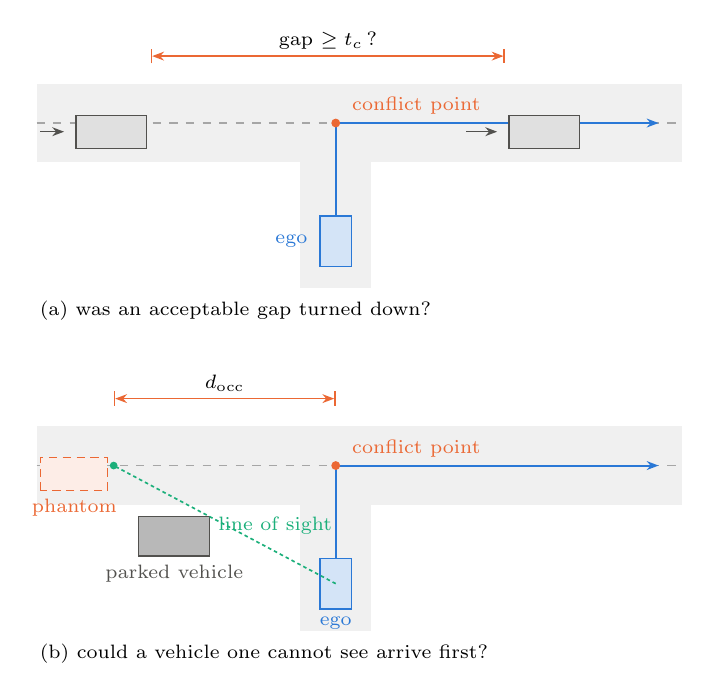
\begin{tikzpicture}[font=\scriptsize,>={Stealth[length=1.5mm]},x=1cm,y=1cm,
  car/.style={draw=fink,fill=black!12,line width=0.45pt},
  ego/.style={draw=fblue,fill=fblue!20,line width=0.55pt}]

% ================= panel (a): gap acceptance =================
\begin{scope}
  \fill[black!6] (0,1.6) rectangle (8.2,2.6);                 % priority road
  \fill[black!6] (3.35,0) rectangle (4.25,1.65);              % minor approach
  \draw[black!35,dashed,line width=0.4pt] (0,2.1) -- (8.2,2.1);
  % ego on the minor approach
  \draw[ego] (3.6,0.28) rectangle (4.0,0.92);
  \node[fblue,anchor=east,inner sep=1.5pt] at (3.5,0.6) {ego};
  \draw[fblue,->,line width=0.7pt] (3.8,0.92) -- (3.8,2.1) -- (7.9,2.1);
  % conflict point
  \fill[forange] (3.8,2.1) circle (1.6pt);
  \node[forange,anchor=south west,inner sep=1.5pt] at (3.95,2.15) {conflict point};
  % priority stream, travelling to the left
  \draw[car] (6.0,1.78) rectangle (6.9,2.2);
  \draw[car] (0.5,1.78) rectangle (1.4,2.2);
  \draw[fink,<-,line width=0.55pt] (5.85,1.99) -- (5.45,1.99);
  \draw[fink,<-,line width=0.55pt] (0.35,1.99) -- (0.05,1.99);
  % the gap between them
  \draw[forange,|<->|,line width=0.55pt] (1.45,2.95) -- (5.95,2.95);
  \node[anchor=south,inner sep=1.5pt] at (3.7,2.98) {gap $\ge t_c$\,?};
  \node[anchor=north west,inner sep=1pt] at (0,-0.12) {(a) was an acceptable gap turned down?};
\end{scope}

% ================= panel (b): blocked sight line =================
\begin{scope}[yshift=-4.35cm]
  \fill[black!6] (0,1.6) rectangle (8.2,2.6);
  \fill[black!6] (3.35,0) rectangle (4.25,1.65);
  \draw[black!35,dashed,line width=0.4pt] (0,2.1) -- (8.2,2.1);
  \draw[ego] (3.6,0.28) rectangle (4.0,0.92);
  \node[fblue,anchor=north,inner sep=1.5pt] at (3.8,0.24) {ego};
  \draw[fblue,->,line width=0.7pt] (3.8,0.92) -- (3.8,2.1) -- (7.9,2.1);
  \fill[forange] (3.8,2.1) circle (1.6pt);
  \node[forange,anchor=south west,inner sep=1.5pt] at (3.95,2.15) {conflict point};
  % an obstruction on the corner, grazed by the line of sight at its far corner
  \draw[car,fill=black!28] (1.3,0.95) rectangle (2.2,1.45);
  \node[fink,anchor=north,inner sep=1.5pt] at (1.75,0.9) {parked vehicle};
  \draw[faqua,line width=0.6pt,dash pattern=on 1.3pt off 1.1pt] (3.8,0.6) -- (0.98,2.1);
  \fill[faqua] (0.98,2.1) circle (1.4pt);
  \node[faqua,anchor=north west,inner sep=1.5pt] at (2.25,1.5) {line of sight};
  % the phantom vehicle, placed just beyond the visible limit
  \draw[forange,densely dashed,fill=forange!12,line width=0.5pt] (0.05,1.78) rectangle (0.9,2.2);
  \node[forange,anchor=north,inner sep=1.5pt] at (0.48,1.74) {phantom};
  \draw[forange,|<->|,line width=0.55pt] (0.98,2.95) -- (3.8,2.95);
  \node[anchor=south,inner sep=1.5pt] at (2.39,2.98) {$d_\mathrm{occ}$};
  \node[anchor=north west,inner sep=1pt] at (0,-0.12) {(b) could a vehicle one cannot see arrive first?};
\end{scope}
\end{tikzpicture}
\caption{The two ways a slow trajectory can be excused. In (a) the ego vehicle
waits while a gap opens in the priority stream; the gap is compared with the
critical gap $t_c$ for that manoeuvre. In (b) no conflicting vehicle is
observed at all, but a parked vehicle cuts the sight line at distance
$d_\mathrm{occ}$ from the conflict point, and a phantom vehicle travelling at
1.1 times the speed limit would arrive before the ego vehicle has cleared.}
\label{fig:geometry}
\end{figure}

\begin{table}[t]
\caption{The tests a candidate has to pass to be labelled over-conservative.
Thresholds carry a literature source; the appendix of the code repository
records the sensitivity runs behind each.}
\label{tab:criteria}
\centering
\footnotesize
\begin{tabular}{@{}ll>{\raggedright\arraybackslash}p{3.15cm}@{}}
\toprule
 & Test & Threshold and source \\
\midrule
\multicolumn{3}{@{}l}{\textit{Is the candidate safe and meaningfully slower?}}\\
O1 & Replay safety & benchmark collision and time-to-collision terms at
                     full marks~\cite{navsim} \\
O2 & Conflict-point margin & post-encroachment time $\ge 1.5$\,s~\cite{allen1978,peesapati2013} \\
O3 & Car-following margin & relative longitudinal envelope, parameters from
                            the reference implementation of~\cite{rss} \\
O4 & Clearly slower & progress ratio to the human drive $\le 0.8$ \\
O5 & Not trivially slow & progress ratio $\ge 0.3$ \\
\addlinespace
\multicolumn{3}{@{}l}{\textit{Is there a reason to be slow?}}\\
O6 & Gap acceptance & critical gap $t_c \in \{4.1, 6.2, 6.5, 7.1\}$\,s by
                      manoeuvre~\cite{hcm6} \\
O7 & Blocked sight line & phantom vehicle at $1.1\,v_\text{lim}$, reaction
                          allowance $1.0$\,s~\cite{orzechowski2018} \\
\bottomrule
\end{tabular}
\end{table}

\subsection{Two kinds of caution, kept apart}
It is worth separating two things that the word conservative covers. A driver
can be slow while crossing, and a driver can refuse to cross at all. On navtest
the human expert almost never does the second: no scene in the interaction
subset shows the expert turning down a gap above the critical value. Yet the
frames we call low-progress are numerous, and there the human's own progress
sub-score is 61.1. Human caution in this data shows up as crossing slowly.
Section~\ref{sec:behaviour} shows that the planner's caution shows up as not
crossing, which is a different mechanism and needs its own measure.

%==============================================================================
\section{Building the Labels}
\label{sec:pipeline}
%==============================================================================

Figure~\ref{fig:pipeline} shows the whole path from a raw log to a training
label. Each stage is described below.

\begin{figure*}[t]
\centering
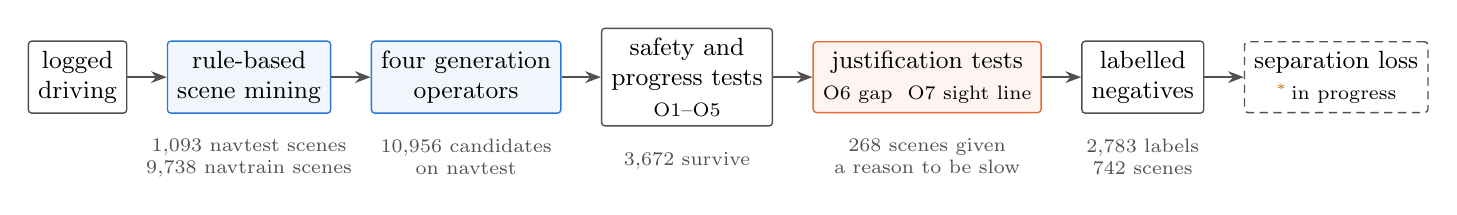
\begin{tikzpicture}[font=\small,>={Stealth[length=2mm]},node distance=4mm,
  box/.style={draw=fink,rounded corners=1.2pt,line width=0.5pt,align=center,
              inner sep=3.5pt,minimum height=8.5mm,fill=white},
  blue/.style={box,draw=fblue,fill=fblue!7},
  orange/.style={box,draw=forange,fill=forange!7},
  lbl/.style={font=\scriptsize,text=fink,align=center}]

\node[box] (logs) {logged\\driving};
\node[blue,right=5mm of logs] (mine) {rule-based\\scene mining};
\node[blue,right=5mm of mine] (gen) {four generation\\operators};
\node[box,right=5mm of gen] (safe) {safety and\\progress tests\\\scriptsize O1--O5};
\node[orange,right=5mm of safe] (just) {justification tests\\\scriptsize O6 gap\ \ O7 sight line};
\node[box,right=5mm of just] (lab) {labelled\\negatives};
\node[box,right=5mm of lab,draw=fink,densely dashed] (train) {separation loss\\\scriptsize\wipnote};

\foreach \a/\b in {logs/mine,mine/gen,gen/safe,safe/just,just/lab,lab/train}
  \draw[->,line width=0.6pt,draw=fink] (\a) -- (\b);

\node[lbl,below=2mm of mine] {1{,}093 navtest scenes\\9{,}738 navtrain scenes};
\node[lbl,below=2mm of gen] {10{,}956 candidates\\on navtest};
\node[lbl,below=2mm of safe] {3{,}672 survive};
\node[lbl,below=2mm of just] {268 scenes given\\a reason to be slow};
\node[lbl,below=2mm of lab] {2{,}783 labels\\742 scenes};
\end{tikzpicture}
\caption{From logs to labels. The two shaded stages are standard: mine the
scenes where the question arises, then perturb the human trajectory into
slower variants. The stage that decides whether a slow variant deserves to be a
negative is the one in orange, and it is where the traffic-engineering
thresholds enter. Counts are for the NAVSIM navtest split.}
\label{fig:pipeline}
\end{figure*}

\subsection{Finding the scenes}
The OpenScene logs behind NAVSIM carry no scenario type, so the subsets are
derived from map geometry. A scene is an unprotected turn when the future path
runs through an unsignalized lane connector whose heading changes by at least
45 degrees. It is a merge when the lane identifier changes inside one roadblock
with a vehicle nearby in the target lane. The third type, an unsignalized
crossing, was added after the merge subset turned out to be small;
Table~\ref{tab:subsets} gives the sizes. Signal control is read from the map
where the attribute exists and from the per-frame signal record otherwise,
because the map interface leaves the turn type and the signalization flag
unimplemented. Four rounds of visual sampling drove the rule revisions.

\begin{table}[t]
\caption{Scene subsets recovered by the geometric rules.}
\label{tab:subsets}
\centering
\footnotesize
\begin{tabular}{@{}lrrr@{}}
\toprule
Subset & navtest & navtrain & share of navtest \\
\midrule
Unprotected turn      & 802   & 6{,}057 & 6.6\% \\
Merge                 & 89    & 1{,}079 & 0.7\% \\
Unsignalized crossing & 205   & 2{,}671 & 1.7\% \\
\midrule
Union                 & 1{,}093 & 9{,}738 & 9.0\% \\
\bottomrule
\end{tabular}
\end{table}

\subsection{Generating slower candidates}
Candidates keep the human path and change only the motion along it, so the
label isolates the timing decision. Table~\ref{tab:operators} lists the
operators. Two of them act on the speed profile, either holding the vehicle at
rest for a moment or scaling the profile down. The other two manufacture a
stop: one halts the vehicle where it had no reason to halt, the other waits out
a conflicting vehicle the human had already passed. An earlier braking operator was dropped
because its effect on four-second progress was negligible, with a median
progress ratio of 0.94.

\begin{table}[t]
\caption{Generation operators and their share of the final navtest labels.}
\label{tab:operators}
\centering
\footnotesize
\begin{tabular}{@{}llrr@{}}
\toprule
 & Operator & Grid & Share \\
\midrule
G1 & Delayed start        & $\Delta t \in \{1.0, 1.5, 2.0\}$\,s & 10.9\% \\
G2 & Scaled speed profile & $\alpha \in \{0.5, 0.65, 0.8\}$     & 45.7\% \\
G3b& Unmotivated stop     & decelerate and hold                 & 42.4\% \\
G4 & Oversized gap        & $\Delta \in \{1.0, 2.0\}$\,s        & 1.0\% \\
\bottomrule
\end{tabular}
\end{table}

\subsection{Filtering}
Figure~\ref{fig:cascade} reports what each test removes. Two observations are
worth drawing out. The progress band is the coarsest filter, cutting 10{,}027
safe candidates to 3{,}699, which is by construction: most perturbations are
not slow enough to matter. The occlusion test is the sharpest of the
justification tests, removing 730 candidates and 221 scenes that every other
test would have kept.

\begin{figure}[t]
\centering
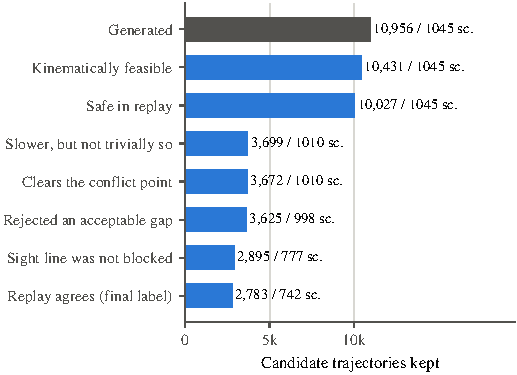
\includegraphics{fig_cascade.pdf}
\caption{Candidates surviving each test, with the number of distinct scenes
they cover. The grey row is the input. Reading the two ends: of 10{,}956
generated candidates, 2{,}783 across 742 scenes become training labels.}
\label{fig:cascade}
\end{figure}

\subsection{The tests do not measure the same thing}
Our original protocol asked for agreement between criteria, on the assumption
that a good label should be confirmed by every test. Measured agreement was
near zero, with pairwise $\kappa$ around 0.08. We now read that result the
other way. The tests are detectors for different excuses, not repeated
measurements of one construct, so low agreement is evidence of independence
rather than of poor quality. Campbell and Fiske's convergent validity applies to
instruments aimed at the same construct~\cite{campbell1959}, which is not our
case, and the $\kappa$ interpretation bands~\cite{mchugh2012} do not transfer.

The useful statistic is coverage. Figure~\ref{fig:complementarity} shows how
many scenes each test protects and how many it protects alone. The blocked
sight line accounts for 244 scenes, and 207 of them are found by no other test.
The replay check finds 41 of its 67 alone. Because the mechanisms barely
overlap, we combine them disjunctively: any test that finds a reason cancels
the label. This errs towards labelling too few, which is the safe direction for
a training signal.

\begin{figure}[t]
\centering
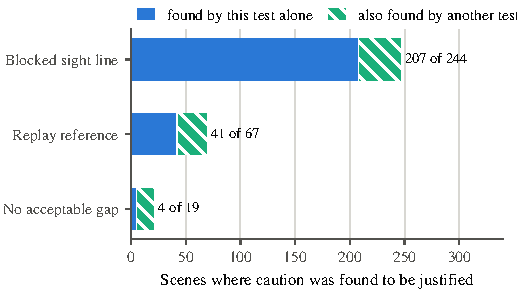
\includegraphics{fig_complementarity.pdf}
\caption{Scenes in which each test finds caution to be justified, split by
whether another test found the same scene. The three tests are close to
disjoint, so dropping any one of them would leave that portion of the scenes
mislabelled.}
\label{fig:complementarity}
\end{figure}

\subsection{Sensitivity}
The most consequential free choice is not a threshold but the rule that decides
which vehicles count as conflicting traffic. Table~\ref{tab:sensitivity} tracks
it. An early rule counted any vehicle passing within 2.5\,m of the ego path,
which swept in queued traffic and inflated justified waiting. Excluding
same-direction vehicles overcorrected, because a right turn onto a major road
conflicts precisely with same-direction traffic. The rule we settled on is
geometric: a vehicle counts when it starts at least 5\,m away from the ego path
and later comes within 2.5\,m, and a vehicle directly behind the ego vehicle is
treated as a follower. Merges are the known weak spot of this rule, since the
conflicting vehicle there is already in the adjacent lane at the start of the
window.

\begin{table}[t]
\caption{Effect of the conflicting-traffic rule on the scene-level verdicts
(navtest, 1{,}045 usable scenes).}
\label{tab:sensitivity}
\centering
\footnotesize
\begin{tabular}{@{}lrrr@{}}
\toprule
Rule & With conflict & Justified wait \\
\midrule
Any vehicle within 2.5\,m          & 489 (47\%) & 224 \\
Same-direction vehicles excluded   & 99 (9.5\%) & 35 \\
\textbf{Entering from outside the path} & \textbf{201 (19\%)} & \textbf{19} \\
\bottomrule
\end{tabular}
\end{table}

%==============================================================================
\section{Measuring the Behaviour}
\label{sec:behaviour}
%==============================================================================

The benchmark score summarises a drive in one number, and the progress term
inside it is normalised against a rule-based planner. When that planner also
waits, a waiting policy is not penalised. We therefore add measures that describe
what the planner did rather than how it scored, all of them decided by the same
tests that produced the labels.

Two of the measures watch stopping. An \emph{unnecessary stop} is a stop of at
least one second that the human did not make, in a scene where no test found a
reason to stop; the \emph{startup delay} is the extra time the planner takes to
move off relative to the human, counted only where the vehicle starts at
rest. The remaining measure watches crossing. The \emph{gap acceptance rate} is
the share of acceptable gaps that the planner takes, restricted to gaps the
human actually used, since otherwise the conflict point lies beyond the
planning horizon and no trajectory could reach it. Replayed through the same
code, the human drive attains the perfect value on every one of them, which is
the sanity check these definitions need.

%==============================================================================
\section{Experiments}
%==============================================================================

\subsection{Setup}
Labels are built on both NAVSIM splits. Evaluation uses the public Latent
TransFuser checkpoints~\cite{transfuser} with three seeds, loaded through a camera-only subclass
because only the navtest camera data fits on the development machine. The full
navtest score of $83.5 \pm 0.45$ reproduces the published 83.8, so the
camera-only path is sound. Confidence intervals are from 10{,}000 bootstrap
resamples over frames.

\subsection{Where the baseline is weak}
Table~\ref{tab:baseline} gives the stratified scores and
Figure~\ref{fig:baseline} the progress term with its interval. Unprotected
turns are the weakest stratum, at 79.2 against 83.5 overall, and their
drivable-area term of 86.4 is the most sensitive safety sub-score in the whole
table. The low-progress stratum is the one the labels target: the planner
scores 58.5 there where the human scores 61.1, so it has reproduced the
human's hesitation almost exactly.

\begin{table}[t]
\caption{Latent TransFuser on navtest, mean over three seeds. Sub-scores are
percentages; PDMS is the composite. The rightmost column is the human drive
replayed through the same scorer.}
\label{tab:baseline}
\centering
\scriptsize
\setlength{\tabcolsep}{3.2pt}
\begin{tabular}{@{}lrrrrrr@{}}
\toprule
Stratum & $n$ & NC & DAC & EP & PDMS & human \\
\midrule
All navtest            & 12{,}146 & 97.7 & 92.3 & 78.3 & 83.5 & 94.8 \\
Unprotected turn       & 802      & 99.9 & 86.4 & 71.3 & 79.2 & 93.4 \\
Merge                  & 89       & 96.8 & 96.3 & 77.4 & 84.1 & 94.5 \\
Unsignalized crossing  & 205      & 99.8 & 100.0& 89.3 & 94.3 & 94.1 \\
Union of the three     & 1{,}093  & 99.6 & 89.7 & 75.1 & 82.5 & 93.6 \\
Low-progress frames    & 198      & 99.7 & 87.2 & 58.5 & 73.9 & 83.8 \\
\bottomrule
\end{tabular}
\end{table}

\begin{figure}[t]
\centering
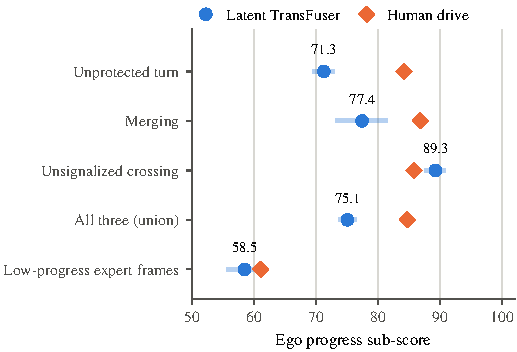
\includegraphics{fig_baseline.pdf}
\caption{Progress sub-score by stratum, with the bootstrap interval over
frames. The gap to the human drive is widest in unprotected turns and closes
almost completely in the low-progress stratum, where the planner has learned
the human's caution.}
\label{fig:baseline}
\end{figure}

\subsection{What the score hides}
Table~\ref{tab:behaviour} is the central empirical result of this paper. Read
it next to Table~\ref{tab:baseline} and the two disagree. Unsignalized
crossings are the planner's best stratum by composite score, at 94.3, and its
best by progress, at 89.3. On gap acceptance the same stratum is the worst in
the table at 30\%. The explanation is the normalisation: the rule-based
reference waits at unsignalized intersections too, so a waiting policy keeps a
high ratio. Figure~\ref{fig:motivation} puts the two views side by side. The
sample behind the crossing figure is ten scenes, so we treat it as indicative
and will recheck it on the larger navtrain split.

A second pattern runs through the table. Startup delay is within $0.2$\,s of
the human everywhere, so the planner is not slow to move off. What it does is
decline to go: about one in five acceptable gaps is refused. This mirrors the
observation in Section~\ref{sec:definition} that human caution takes the
opposite form, and it says that a measure of hesitation built around reaction
time would have found nothing here.

\begin{figure}[t]
\centering
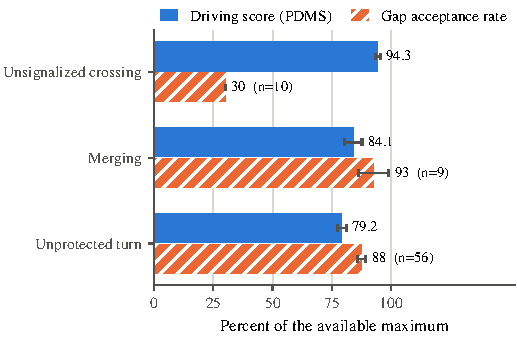
\includegraphics{fig_motivation.pdf}
\caption{The benchmark score and gap acceptance disagree. Unsignalized
crossings earn the highest composite score of any stratum while the planner
takes fewer than a third of the gaps a human took there. Bars show the mean over
three seeds; whiskers are the bootstrap interval for the score and the seed
spread for gap acceptance.}
\label{fig:motivation}
\end{figure}

\begin{table}[t]
\caption{Behaviour measures for the baseline, mean over three seeds with the
seed spread. The human drive attains the perfect value in every column by construction.}
\label{tab:behaviour}
\centering
\scriptsize
\setlength{\tabcolsep}{4pt}
\begin{tabular}{@{}lrrr@{}}
\toprule
Stratum & Unnecessary & Startup & Gap acceptance \\
        & stops (\%)  & delay (s) & (\%, eligible $n$) \\
\midrule
Union of the three    & $1.53 \pm 0.29$ & $-0.01 \pm 0.03$ & $80.4 \pm 0.8$ (75) \\
Unprotected turn      & $0.09 \pm 0.08$ & $+0.14 \pm 0.07$ & $87.5 \pm 1.8$ (56) \\
Merge                 & $6.13 \pm 0.66$ & $+0.05 \pm 0.01$ & $92.6 \pm 6.4$ (9) \\
Unsignalized crossing & $5.31 \pm 1.52$ & $-0.04 \pm 0.03$ & $\mathbf{30.0 \pm 0.0}$ (10) \\
\bottomrule
\end{tabular}
\end{table}

\subsection{Label yield}
The final navtest label set holds 2{,}783 trajectories over 742 scenes; navtrain
holds 20{,}799 over 5{,}819. Adding the occlusion test cut the navtest set by
roughly a fifth and the navtrain set by a quarter, which is the price of not
punishing caution that the sight line justified. Scenes where a vehicle was
hidden are far more common in unsignalized crossings than in turns, at 55\%
against 22\% on navtrain, matching the intuition that a crossing is the
manoeuvre most exposed to what one cannot see.

%==============================================================================
\section{Training: Work in Progress}
\label{sec:wip}
%==============================================================================

The labels exist to be trained on, and that step is not finished. The 8\,GB
development machine cannot hold the sensor data for navtrain, so training runs
on a separate machine that is being provisioned. This section records the design
and the acceptance criteria so that the result can be checked against a
prediction rather than described after the fact.

For a regression planner the auxiliary term is a margin loss that pushes the
prediction away from a labelled negative relative to the human trajectory,
$L_\text{neg} = \max\!\left(0,\; m - \bigl(d(\hat\tau,\tau_\text{neg}) -
d(\hat\tau,\tau^{*})\bigr)\right)$, with $d$ the mean waypoint distance. The
total loss adds it to the imitation loss with a weight below one, active only on
frames that carry a label. A contrastive variant is implemented for ablation.
For a scoring planner the label instead marks the nearest vocabulary trajectory
as a hard negative and adds a ranking term.

The acceptance criterion is stated in advance. In the interaction subset the gap
acceptance rate must rise and the unnecessary-stop rate must fall, while the
lower bound of the bootstrap interval on every safety sub-score stays at or
above the baseline mean. In scenes where a test found caution justified, the gap
acceptance rate must \emph{not} rise, since a rise there would mean the model
learned to be reckless rather than decisive.

Two further pieces are pending. The braking operator still yields almost nothing
and needs redesigning\wip. Transfer to a vector-input planner in closed-loop
simulation is planned after the open-loop result settles\wip.

%==============================================================================
\section{Limitations}
%==============================================================================

The occlusion test sees only vehicles as obstructions, because the map carries
no buildings. It therefore understates how often the view is blocked, and the
bias runs towards keeping labels that a fuller model would have removed.
Phantom speed comes from the posted limit, with a default where the map omits
it.

The gap test degrades on merges, where the conflicting vehicle is already
alongside at the start of the window and so fails the entering-from-outside
rule. Safety there rests on the replay check and the car-following margin. The
right measure for a merge is the headway in the target lane, which we have not
implemented.

Replay is non-reactive. Other vehicles in the log have already yielded to the
real, more cautious ego vehicle, so a faster reference trajectory rarely
triggers a collision. This is why the replay check rejects only a small
fraction on its own and why we did not rely on it alone.

Finally, the numbers in Table~\ref{tab:behaviour} rest on small eligible
samples in two strata. They are reported with their sample sizes and should be
read as a direction to check, not as a settled effect.

%==============================================================================
\section{Conclusion}
%==============================================================================

Waiting when there is no reason to wait is a failure mode that current training
signals do not name and current benchmark scores do not see. We gave it a
definition that a machine can evaluate, built from gap thresholds that traffic
engineering has measured and from a reachability argument about vehicles the ego
cannot see. Applied to NAVSIM the definition yields 2{,}783 labelled
trajectories on navtest without any human annotation, and the two justification
tests turn out to protect almost disjoint sets of scenes, so both are needed.
Measuring the baseline against these labels showed a planner that scores best
exactly where it hesitates most, which is the clearest argument we can give for
not reading the composite score alone. Whether training on the labels moves the
behaviour is the next question, and the criterion for answering it is fixed in
advance in Section~\ref{sec:wip}.

\section*{Acknowledgment}
The first author thanks the members of the Nakano laboratory for discussion of
the scene definitions.

\bibliographystyle{IEEEtran}
\bibliography{refs}

\end{document}
